\section{Visualization of TensorFlow Graphs}\label{sec:visual}

Deep learning models often employ neural networks with a highly complex and
intricate structure. For example, \cite{inception} reports of a deep
convolutional network based on the Google \emph{Inception} model with more than
36,000 individual units, while \cite{tensorflow} states that certain long
short-term memory (LSTM) architectures can span over 15,000
nodes. \emph{TensorBoard}, a web interface for graph visualization built
directly into TensorFlow, allows the user to maintain a clear overview of such
complex structures and facilitates model debugging.

The core feature of TensorBoard is the lucid visualization of computational
graphs, exemplified in Figure \ref{fig:tensorboard-a}. Graphs with complex
topologies and many layers can be displayed in a clear and organized manner,
allowing the user to understand exactly how data flows through it. Especially
useful is TensorBoard's notion of \emph{name scopes}, whereby nodes or entire
subgraphs may be grouped into one visual block, such as a single neural network
layer. Such name scopes can then be expanded interactively to show the grouped
units in more detail. Figure \ref{fig:tensorboard-b} shows the expansion of one
the name scopes of Figure \ref{fig:tensorboard-a}.

Furthermore, TensorBoard allows the user to track the development of individual
tensor values over time. For this, you can attach two kinds of \emph{summary
  operations} to nodes of the computational graph: \emph{scalar summaries} and
\emph{histogram summaries}. Scalar summaries show the progression of a scalar
tensor value, which can be sampled at certain iteration counts. In this way, you
could, for example, observe the accuracy or loss of your model with
time. Histogram summary nodes allow the user to track value
\emph{distributions}, such as those of neural network weights or the final
softmax estimates. Figures \ref{fig:tensorboard-c} and \ref{fig:tensorboard-d}
give examples of scalar and histogram summaries, respectively. Lastly,
TensorBoard also allows visualization of images. This can be useful to show the
images sampled for each mini-batch of an image classification task, or to
visualize the kernel filters learned for a convolutional neural network
\cite{tensorflow}.

\begin{figure}[h!]
  \centering
  \begin{subfigure}[h]{0.5\textwidth}
    \centering
    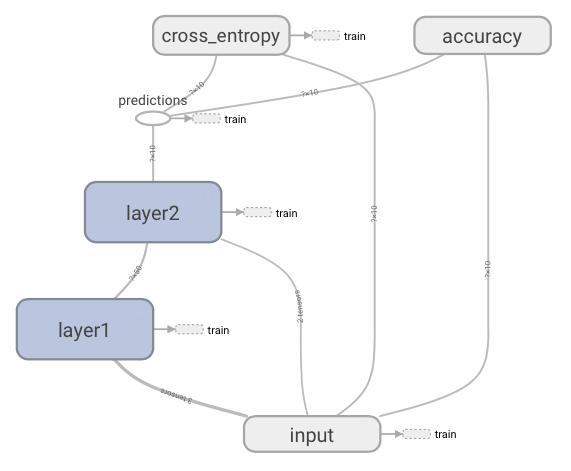
\includegraphics[scale=0.4]{no-train}
   \caption{}
   \label{fig:tensorboard-a}
  \end{subfigure}

  \vspace{0.3cm}

  \begin{subfigure}[h]{0.5\textwidth}
    \centering
    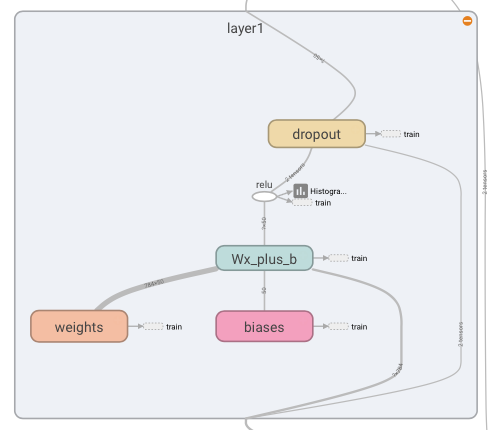
\includegraphics[scale=0.4]{layer1}
    \caption{}
    \label{fig:tensorboard-b}
  \end{subfigure}

  \vspace{0.3cm}

  \begin{subfigure}[h]{0.2\textwidth}
    \centering
    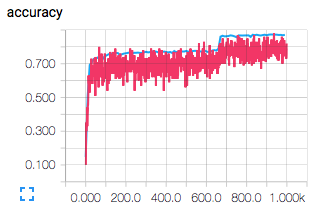
\includegraphics[scale=0.35]{accuracy}
    \caption{}
    \label{fig:tensorboard-c}
  \end{subfigure}
  %
  \begin{subfigure}[h]{0.2\textwidth}
    \centering
    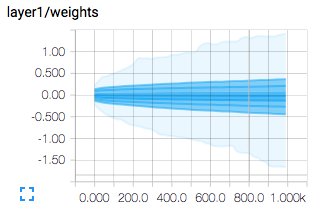
\includegraphics[scale=0.35]{blue-weights}
    \caption{}
    \label{fig:tensorboard-d}
  \end{subfigure}
  \caption{A demonstration of TensorBoard's graph visualization features. Figure
    \ref{fig:tensorboard-a} shows the complete graph, while Figure
    \ref{fig:tensorboard-b} displays the expansion of the first layer. Figures
    \ref{fig:tensorboard-c} and \ref{fig:tensorboard-d} give examples for scalar
    and histogram summaries, respectively.}
  \label{fig:tensorboard}
\end{figure}

%%% Local Variables:
%%% mode: latex
%%% TeX-master: "../paper"
%%% End: